\documentclass[a4paper,11pt]{article} 
\usepackage{latexsym} 
\usepackage[MeX]{polski} 
\usepackage{indentfirst}
\usepackage{graphicx}
\usepackage[utf8]{inputenc} 


\author{Bartosz Michałowski} 
\title{
	\Huge Specyfikacja funkcjonalna \\
	automat komórkowy\\
	\textbf{"Wire World"}
} 
\frenchspacing 
\begin{document} 
	\maketitle 
	\newpage
	\tableofcontents 
	\newpage
	\section {Opis ogólny}
	\subsection{Nazwa programu} 
	Nazwa programu:~\texttt{WireWorld}
	\subsection{Poruszany problem}
	Automatem komórkowym określa się system składający się z pojedynczych komórek, znajdujących się obok siebie. Każda z~komórek może przyjąć jeden ze stanów, przy czym liczba stanów jest skończona, ale dowolnie duża. Stan komórek zmieniany jest synchronicznie w~zależności od komórek otaczających oraz przyjętych reguł. Poruszanym problemem jest implementacją takowego automatu komórkowego \textbf{Wire World} autorstwa Briana Silvermana i~stworzenie modułu wizualizującego planszę w~czasie rzeczywistym. Program zostanie napisany w języku \textbf{Java}. W programie nie przewiduje się zastosowania konstrukcji dostępnych w \textbf{Javie wersji~8} i~wyższej. 
	\newpage
	\section{Opis funkcjonalności}
		\subsection{Wymagania funkcjonalne}
		\begin{itemize}
		\item Wczytywanie do programu początkowej konfiguracji z~pliku o~wybranym formacie
		\item Przeprowadzanie żądanej liczby generacji.
		\item Wizualizacja w~czasie rzeczywistym zmieniając generacje ręcznie lub włączając tryb auto-przełączania
		\item Zapisanie bieżącej generacji do pliku, który może być później wczytany
		\item Tworzenie i~edytowanie generacji w trybie rzeczywistym za pomocą interfejsu graficznego
		\item Wstawianie gotowych struktur odpowiadających za bardziej zaawansowane struktury
	  \end{itemize}
	  \subsection{Jak korzystać z programu}
	Obsługę programu umożliwia intuicyjny i~czytelny interfejs graficzny. Jest on przeznaczony do wczytania z~pliku odpowiedniej generacji komórek, narysowania jej ręcznie, bądź edytowania bieżącej. Z~poziomu interfejsu użytkownik może importować gotowe struktury i~sterować przebiegiem procesu generacji. Przez proces ten rozumie się przeprowadzenie symulacji, przechodzenie pomiędzy kolejnymi stanami i~definiowanie określonych atrybutów, takich jak rozmiary planszy, czy miejsce zapisu wybranej generacji.
	  \subsection{Uruchomienie programu}
	Program przeznaczony jest do uruchomiania za pomocą pliku \texttt{WireWorld.jar}.
			
	\newpage
	\section{Opis danych wejściowych i~interfejsu} 
		\subsection{Struktura pliku wejściowego}
			W Wireworld wyróżniamy następujące stany komórek:
			\begin{itemize}
			  \item \texttt{EMPTY} pusta komórka 
			  \item \texttt{CONDUCTOR} komórka przewodząca elektrony
			  \item \texttt{HEAD} głowa elektronu
			  \item \texttt{TAIL} ogon elektronu
			\end{itemize}
			Oraz następujące struktury:
			\begin{itemize}
			  \item \texttt{ELECTRON} elektron 
			  \item \texttt{DIODE} dioda
			  \item \texttt{OR} bramka logiczna OR
			  \item \texttt{AND} bramka logiczna AND
			  \item \texttt{XOR} bramka logiczna XOR
			  \item \texttt{CLOCK} prosty generator elektronów 
			\end{itemize}
			Plik tekstowy musi zawierać w pierwszej kolejności wymiary planszy, na~której przeprowadzane będą generacje, jako dwie kolejne liczby całkowite. Następnie w oddzielnych liniach należy zamieścić instrukcje modyfikujące komórki siatki zgodnie z następującym wzorcem:
			\begin{center}
			\texttt{NAZWA\_STRUKTURY/STANU POZYCJA\_X POZYCJA\_Y ORIENTACJA}
			\end{center}
			Orientacja jest argumentem opcjonalnym i~dostępnym jedynie dla struktur, a~w~wypadku próby przypisania jej do stanu zostanie ona pominięta. Za~rotacje odpowiadają następujące wartości argumentu:
			\begin{itemize}
			  \item \textbf{L} struktura zwrócona w stronę lewej krawędzi siatki
			  \item \textbf{U} struktura zwrócona w stronę górnej krawędzi siatki
			  \item \textbf{R} struktura zwrócona w stronę prawej krawędzi siatki
			  \item \textbf{D} struktura zwrócona w stronę dolnej krawędzi siatki
			\end{itemize}
			Domyślnie struktury zwrócone są w stronę prawej krawędzi planszy. 
		\subsection{Przechowywanie danych w programie}
				Wszelkie informacje w~programie przechowywane są w~polach obiektów odpowiednich klas.
		\subsection{Dane wyjściowe }
				Z~poziomu interfejsu graficznego istnieje możliwość stworzenia pliku zawierający wybraną generacje w~formie analogicznej do formy pliku wejściowego, w~miejscu zdefiniowanym przez użytkownika.
		\subsection{Interfejs graficzny}
			Interfejs graficzny daje użytkownikowi szeroki zakres opcji umożliwiających modyfikacje warunków w~jakich nastąpi generacja. Należą do nich:
			\begin{itemize}
			  \item Wczytywanie pierwszej generacji z~pliku
			  \item Tworzenie pierwszej generacji z~dostępnych elementów
			  \item Wybór liczby pożądanych generacji
			  \item Zapisanie aktualnego stanu siatki do pliku
			  \item Poruszanie się po kolejnych generacjach
			  \item Automatyczne przechodzenie przez generacje przy wybranej prędkości
			  \begin{figure}[h]
			    \begin{center}
			      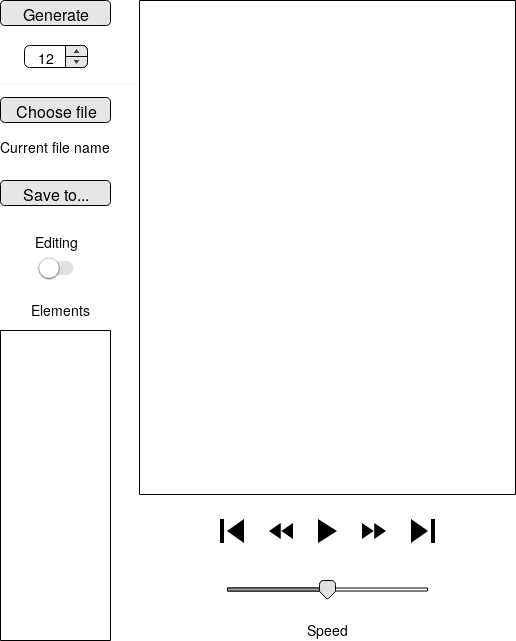
\includegraphics[scale=0.5]{GUI.png}
			      \caption{Szkic poglądowy interfejsu graficznego}
			      \label{fig:}
			    \end{center}
			  \end{figure}
			\end{itemize}
		\newpage
		\section{Komunikaty dla użytkownika i~testowanie}
		  \subsection{Przykładowe komunikaty skierowane do użytkownika}
				    \begin{itemize}
				      \item Pomyślnie utworzono generację
				      \item Nie udało się wczytać pliku wejściowego - spowodowane brakiem uprawnień
				      \item Nie udało się utworzyć pliku wyjściowego - spowodowane brakiem uprawnień
				      \item Błędny format pliku wejściowego - plik wejściowy zawiera niedozwolone znaki
				    \end{itemize}
			\subsection{Ogólny przebieg testowania}
	Na ogół procesów testowania będą składały  się odpowiednie fazy testowe. Pozwolą one w~sposób optymalny sprawdzać tworzony program. Wodzącymi narzędziami użytymi do weryfikowania kodu będą \texttt{JUnit} i~\texttt{AssertJ}. Interfejs graficzny zostanie sprawdzony ręcznie, podczas tworzenia programu. Celem procesu testowania jest zapewnienie obsługi zdarzeń, w~których program może zachowywać się w~sposób niekontrolowany.
\end{document}
